%-------------------------------------------
%\thispagestyle{empty}\cleardoublepage
%\phantomsection
%\addcontentsline{toc}{chapter}{Tutorials}
\chapter*{Tutorials}
%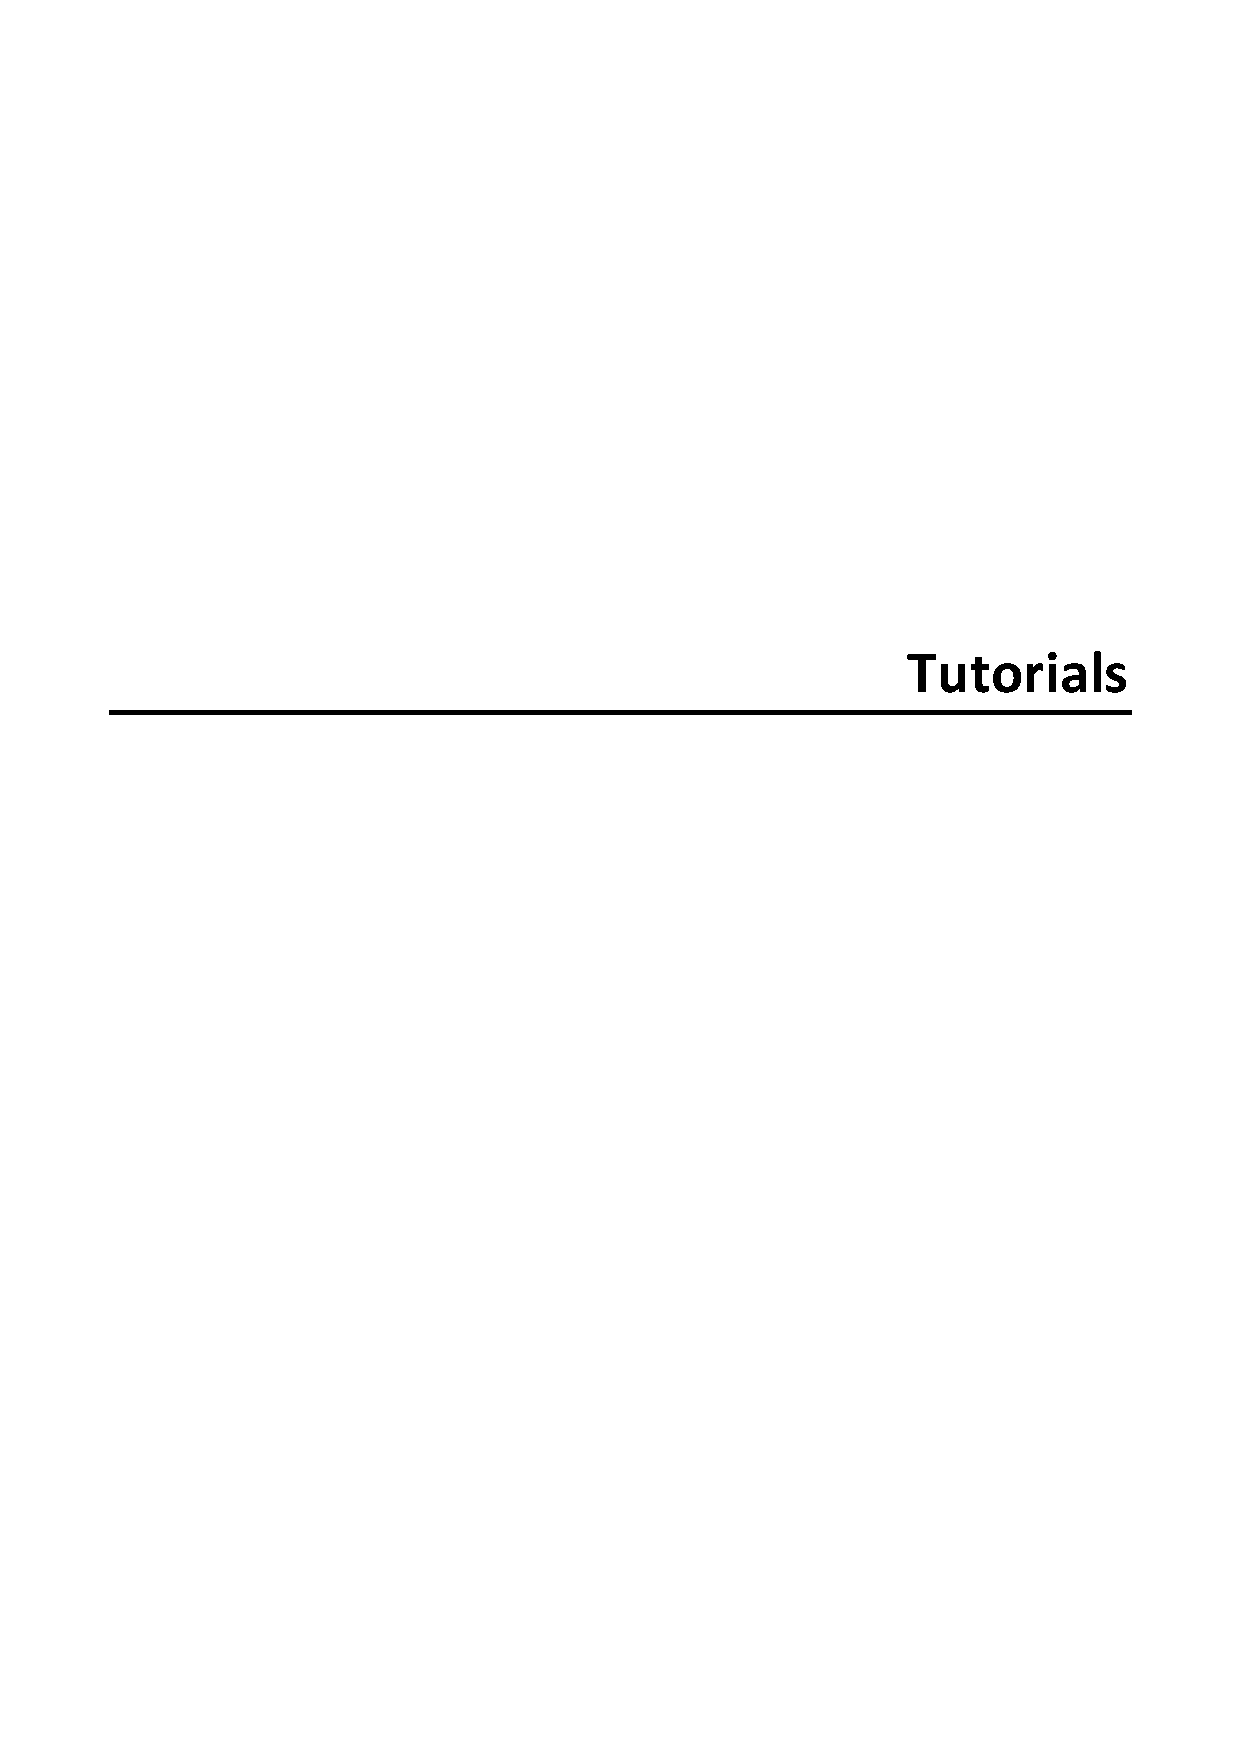
\includepdf[pages=1,pagecommand=\thispagestyle{empty}]{external/11_Tutorials_SectionDivider.pdf}
\thispagestyle{empty}\cleardoublepage
 %-------------------------------------------


% Tutorial 1
\section*{Tutorial 1}
\phantomsection
\addcontentsline{toc}{section}{Analysing Physiological Data Collected During Music Listening: 
An Introduction
\texorpdfstring{\\\textit{Laura Bishop, Geoffray Bonnin and Jérémy Frey}}{}}
%\includepdf[pages=1, pagecommand=\thispagestyle{fancy}]{external/11_Tutorials.pdf}
\subsection*{Analysing Physiological Data Collected During Music Listening: 
An Introduction}
\speaker{Laura Bishop, Geoffray Bonnin and Jérémy Frey}

\subsection*{Abstract}
Music has diverse effects on listeners, including inducing emotions, triggering movement or dancing, and prompting changes in visual attention. These effects are often associated with psychophysiological responses like changes in heart activity, respiratory rate, and pupil size, which can themselves be influenced by the cognitive effort exerted during music listening, e.g., when engaging with unfamiliar tracks on a web radio for music discovery.

This tutorial aims to introduce psychophysiological data analysis for a broad MIR audience, with a particular focus on the analysis of heart rate, electrodermal activity and pupillometry data. It will be structured in three parts. The first part will provide a presentation of psychophysiological data that we collected in the context of a preliminary study related to music discovery. The second part will be a hands-on tutorial during which we will guide the participants to remake two of our data analyses. In the third part, we will assist participants in undertaking their own data analysis of our data. These analyses will be demonstrated using R and Python.

Our aim with this tutorial is twofold: to promote underrepresented topics in the MIR community, especially the recognition of induced emotions from physiological data and discovery-oriented music recommendation; and to encourage researchers from those domains to interact with the MIR community. The audience we target is therefore relatively large. Participants should, however, possess sufficient knowledge of R and/or Python and standard statistical analysis methods to participate in the hands-on parts of the tutorial.

\subsection*{Biographies of the Presenters}
\paragraph*{Laura Bishop} is a researcher at the RITMO Centre for Interdisciplinary Studies in Rhythm, Time and Motion and the Department of Musicology at the University of Oslo. She specialises in pupillometry, eye-tracking, and motion capture using approaches mainly grounded in psychology. She completed her PhD in music psychology at the MARCS Institute, Western Sydney University, Australia, in 2013. She currently co-leads the Austrian Science Fund project ``Achieving togetherness in music ensembles'' in collaboration with the University for Music and Performing Arts Vienna (mdw), which investigates physiological and body motion coordination in ensemble playing.

\paragraph*{Geoffray Bonnin} is an Associate Professor at the Lorraine Research Laboratory in Computer Science and its Applications (Loria), Université de Lorraine. He obtained his Ph.D. in 2010 and joined the Loria lab in 2014 as an Associate Professor. His research topics are related to artificial intelligence for music and for education. He is currently in charge of the Music-Mouv' project, which is a collaboration with researchers in the domain of psychology that started in October 2021. The project aims at helping individuals with Parkinson's disease to walk by triggering relevant emotions through physiology-based music recommendations.

\paragraph*{Jérémy Frey} is the CTO and co-founder of Ullo. After a master degree in cognitive sciences, he obtained his PhD degree in computer science in 2015 from the University of Bordeaux, France. During his work within the Inria research team Potioc, he had been studying how passive brain-computer interfaces could contribute to the evaluation of user experience, using for example EEG to infer a continuous index of cognitive load. His current research interests revolve around increasing introspection and social presence, by displaying inner states through tangible interfaces or wearables, with applications ranging from well-being to education.

\clearpage


% Tutorial 2
\section*{Tutorial 2}
\phantomsection
\addcontentsline{toc}{section}{Introduction to Differentiable Audio Synthesizer Programming
\texorpdfstring{\\\textit{Ben Hayes, Jordie Shier, Chin-Yun Yu, David Südholt and Rodrigo Diaz}}{}}
%\includepdf[pages=2-3, pagecommand=\thispagestyle{fancy}]{external/11_Tutorials.pdf}
\subsection*{Introduction to Differentiable Audio Synthesizer Programming}
\speaker{Ben Hayes, Jordie Shier, Chin-Yun Yu, David Südholt and Rodrigo Diaz}

\subsection*{Abstract}
Differentiable digital signal processing is a technique in which signal processing algorithms are implemented as differentiable programs used in combination with deep neural networks. The advantages of this methodology include a reduction in model complexity, lower data requirements, and an inherently interpretible intermediate representation. In recent years, differentiable audio synthesizers have been applied to a variety of tasks, including voice and instrument modelling, synthesizer control, pitch estimation, source separation, and parameter estimation. Yet despite the growing popularity of such methods, the implementation of differentiable audio synthesizers remains poorly documented, and the simple formulation of many synthesizers belies their complex optimization behaviour. To address this gap, this tutorial offers an introduction to the fundamentals of differentiable synthesizer programming.

The tutorial will centre around practical demonstrations, which participants can follow using an accompanying suite of Jupyter notebooks. All tutorial content will be documented in an accompanying web book, and all tutorial materials and dependencies will be fully open source and accessible for free online. Prior experience with writing Python 3 code is assumed, and a basic knowledge of PyTorch is beneficial though not strictly required. The tutorial is targeted at music and audio researchers and engineers with a grounding in the basics of digital signal processing and machine learning. Our aim is to equip participants to apply these techniques in their own research, whilst enabling those with prior knowledge to sharpen their skills.


\subsection*{Biographies of the Presenters}
\paragraph{Ben Hayes} is a third year PhD student at the Centre for Digital Music's CDT in Artificial Intelligence and Music, based at Queen Mary University of London, under the supervision of Dr György Fazekas and Dr Charalampos Saitis. His research focuses on expanding the capabilities of differentiable digital signal processing by enabling control over non-convex operations. His work has been accepted to leading conferences in the field, including ISMIR, ICASSP, ICA, and the AES Convention, and published in the Journal of the Audio Engineering Society. He also holds an MSc with Distinction in Sound and Music Computing from QMUL and a first class BMus(Hons) in Electronic Music from the Guildhall School of Music and Drama, where he is now a member of teaching faculty. He is a founding member of the Special Interest Group on Neural Audio Synthesis at C4DM, and is the organizer of the international Neural Audio Synthesis Hackathon. Previously he was a Research intern at ByteDance, music lead at the award-winning generative music startup Jukedeck, and an internationally touring musician signed to R\&S Records.

\paragraph{Jordie Shier} is a first year PhD student in the Artificial Intelligence and Music (AIM) programme based at Queen Mary University of London (QMUL), studying under the supervision of Prof. Andrew McPherson and Dr. Charalampos Saitis. His research is focused on the development of novel methods for synthesizing audio and the creation of new interaction paradigms for music synthesizers. His current PhD project is on real-time timbral mapping for synthesized percussive performance and is being conducted in collaboration with Ableton. He was a co-organizer of the 2021 Holistic Evaluation of Audio Representations (HEAR) NeurIPS challenge and his work has been published in PMLR, DAFx, and the JAES. Previously, he completed an MSc in Computer Science and Music under the supervision of Prof. George Tzanetakis and Assoc. Prof. Kirck McNally.

\paragraph{Chin-Yun Yu} is a first year PhD student in the Artificial Intelligence and Music (AIM) programme based at Queen Mary University of London (QMUL), under the supervision of Dr György Fazekas. His current research theme is on leveraging signal processing and deep generative models for controllable, expressive vocal synthesis. In addition, he is dedicated to open science and reproducible research by developing open-source packages and contributing to public research projects. He received a BSc in Computer Science from National Chiao Tung University in 2018 and was a research assistant at the Institute of Information Science, Academia Sinica, supervised by Prof. Li Su. His recent work has been published at ICASSP.

\paragraph{David Südholt} is a first year PhD student in the Artificial Intelligence and Music (AIM) programme based at Queen Mary University of London (QMUL). Supervised by Prof. Joshua Reiss, he is researching parameter estimation for physical modelling synthesis, focussing on the synthesis and expressive transformation of the human voice. He received an MSc degree in Sound and Music Computing from Aalborg University Copenhagen in 2022, where he was supervised by Prof. Stefania Serafin and Assoc. Prof. Cumhur Erkut. His work has been published at the SMC conference and in the IEEE/ACM Transactions on Audio, Speech and Language Processing.

\paragraph{Rodrigo Diaz} is a PhD candidate in Artificial Intelligence and Music at Queen Mary University in London, under the supervision of Prof. Mark Sandler and Dr. Charalampos Saitis. Rodrigo's work has been published in leading computer vision and audio conferences, including CVPR, ICASSP, IC3D, and the AES Conference on Headphone Technology. Before starting his PhD studies, he worked as a researcher at the Immersive Communications group at the Fraunhofer HHI Institute in Berlin, where he investigated volumetric reconstruction from images using neural networks. His current research focuses on real-time audio synthesis using neural networks for 3D objects and drums. Rodrigo's interdisciplinary background includes a Master's degree in Media Arts and Design from Bauhaus University in Weimar and a Bachelor of Music from Texas Christian University.

\clearpage


% Tutorial 3
\section*{Tutorial 3}
\phantomsection
\addcontentsline{toc}{section}{Transformer-Based Symbolic Music Generation: Fundamentals to Advanced Concepts, Stylistic Considerations, Conditioning Mechanisms and Large Language Models
\texorpdfstring{\\\textit{Berker Banar, Pedro Sarmento and Sara Adkins}}{}}
%\includepdf[pages=4-5, pagecommand=\thispagestyle{fancy}]{external/11_Tutorials.pdf}
\subsection*{Transformer-Based Symbolic Music Generation: Fundamentals to Advanced Concepts, Stylistic Considerations, Conditioning Mechanisms and Large Language Models}
\speaker{Berker Banar, Pedro Sarmento and Sara Adkins}

\subsection*{Abstract}
With the rise of the attention mechanism and the success of auto-regressive generative modelling and large language models, the Transformer architecture has arguably been the most promising technology for symbolic music generation. While audio-based methods have shown promise, symbolic music generation offers distinct advantages in terms of control, long-term coherence and computational efficiency. This tutorial explores the potential of the Transformer architecture in symbolic music generation and aims to provide (1) a thorough understanding of the vanilla Transformer architecture (emphasising the reasoning behind its design choices) and the utilisation of large language models for symbolic music generation. Additionally, it offers (2) a comprehensive overview of the field, including a taxonomy and a curated list of valuable datasets. The tutorial delves into (3) an in-depth analysis of Transformer variants and large language models specifically tailored for symbolic music generation. Also, it examines (4) examples and advanced considerations such as style, musical conditioning, and real-time performance. Furthermore, the tutorial offers (5) two hands-on exercises using Google Colab Notebooks, enabling participants to apply the concepts covered. Overall, this tutorial equips participants with the theoretical knowledge and practical skills necessary to explore the power of the Transformer architecture in symbolic music generation.

\subsection*{Biographies of the Presenters}
\paragraph{Berker Banar} is a PhD Researcher (Comp. Sci.) at the Centre for Doctoral Training in AI and Music (AIM CDT) and the Centre for Digital Music (C4DM) at Queen Mary University of London (QMUL), and also an Enrichment Student at the Alan Turing Institute. His PhD focuses on `Composing Contemporary Classical Music using Generative Deep Learning' under supervision of Simon Colton to enhance human creativity and enable new aesthetics. Berker's research interests include transformer-based generative modelling, optimisation, self-supervised representation learning for audio and music, explainable AI, quality-diversity analysis of generative model and out-of-distribution generation. He has worked at Sony and Bose as a research intern, and at Northwestern University Metamaterials and Nanophotonic Devices Lab as a nanophotonics researcher. Berker holds a BS in Electrical and Electronics Engineering from Bilkent University, Ankara, Turkey and a BM in Electronic Production and Design from Berklee College of Music, Boston, MA. His awards include Enrichment Community Award (The Alan Turing Institute), Exceptional Great Work Award (Bose), Outstanding Students of 2022 (EvoMUSART), Roland Award Endowed Scholarship (Berklee) and Outstanding Success Scholarship (Turkish Educational Foundation, upon ranking 17th in 1.5 million people in national university entrance exam). As a musician (drums and electronics), Berker has performed at venues such as the Museum of Fine Arts Boston, Harvard University Holden Chapel \& Carpenter Center for Visual Arts (an original piece premiered as part of Berklee Interdisciplinary Arts Institute), Berklee Performance Center, Wally's Jazz Club Boston, Nardis Jazz Club Istanbul and Istanbul Jazz Festival.

\paragraph{Pedro Sarmento} is a PhD researcher at the Centre for Digital Music (C4DM), Queen Mary University of London (QMUL), working under the supervision of Mathieu Barthet within the UKRI Centre for Doctoral Training in Artificial Intelligence and Music (AIM). His research focuses on guitar-focused symbolic music generation with deep learning. This concerns the exploration of techniques for the creation of novel music that is represented in a digital tablature format, in which additional information about how to play specific music passages is provided. He holds an Integrated MSc degree in Electrical Engineering from Faculdade de Engenharia da Universidade do Porto (FEUP), a degree in Classical Guitar from the Conversatory of Music of Porto, and a second MSc degree in Multimedia and Interactive Sound from FEUP. He has an ongoing collaboration with Orquestra de Jazz de Matosinhos (OJM) where he leads sessions that foster an approach to STEM via musical concepts for young students. He volunteers for an online music magazine, writing album reviews and conducting interviews with artists from the Metal scene.

\paragraph{Sara Adkins} is a music technologist, machine learning engineer, and performer who is enthusiastic about promoting the use of machine learning and AI in the creative arts. Currently, she works as a Generative Music and Audio Developer at Infinite Album, developing a real-time, interactive, and copyright-safe music engine for Twitch streamers. Sara holds a Master of Science in Sound and Music Computing from Queen Mary University of London where she was funded through a US-UK Fulbright grant. Her master's thesis focused on developing a Transformer model capable of generating loopable musical phrases for live coding and algorave performances, and received an Outstanding Student Mention at EvoMUSART 2023. Before moving to London, Sara spent three years in Boston where she worked as a machine learning engineer at Bose and played as a freelance classical guitarist. At Bose, she worked on deep learning models for speech enhancement that were optimized to run live on a hearing aid micro-controller. She also led a research project that developed generative audio algorithms that adapt to biofeedback signals to induce sleep using soothing music. Sara graduated from Carnegie Mellon University with an interdisciplinary bachelor's degree in music technology and computer science. Her senior capstone project, ``Creating with the Machine,'' combined algorithmic and traditional methods of composition into live performances to explore how interactive generative algorithms can influence creativity in musical improvisation. ``Creating with the Machine'' was premiered by the Carnegie Mellon Exploded Ensemble in the spring of 2018 and was awarded the Henry Armero Memorial Award for Inclusive Creativity.

\clearpage


% Tutorial 4
\section*{Tutorial 4}
\phantomsection
\addcontentsline{toc}{section}{Computer-Assisted Music-Making Systems: Taxonomy, Review, and Coding
\texorpdfstring{\\\textit{Christodoulos Benetatos, Zhiyao Duan and Philippe Pasquier}}{}}
%\includepdf[pages=6, pagecommand=\thispagestyle{fancy}]{external/11_Tutorials.pdf}
\subsection*{Computer-Assisted Music-Making Systems: Taxonomy, Review, and Coding}
\speaker{Christodoulos Benetatos, Zhiyao Duan and Philippe Pasquier}

\subsection*{Abstract}
Computer-Assisted Music-Making (CAMM) systems, are software-based tools designed to assist and augment the musical creativity of composers, performers, and music enthusiasts. CAMM systems encompass a wide range of systems that can be broadly categorized into two main types according to their design purposes: to assist music performance and to assist music composition. This tutorial offers a comprehensive review of the design principles, practical applications, taxonomy, and the state-of-the-art research of CAMM systems, with an emphasis on systems assisting music performance, which are also called ``interactive music systems'' or ``musical agents'' in the literature. Research on CAMMs is interdisciplinary in its nature, combining fields such as Music Information Retrieval (MIR), Artificial Intelligence (AI) and Human-Computer Interaction (HCI). Participants will gain an understanding of how these fields converge to create innovative and interactive musical experiences. This tutorial will also feature a coding session for participants to build a real-time musical agent, under the framework of Euterpe, a prototyping framework for creating music interactions on the Web. The tutorial will examine existing systems built using Euterpe, provide insights into the development process, and guide participants through the creation of their own musical agents. Participants in the coding part should bring a laptop with Chrome and Node.js (\href{https://nodejs.org/en/download}{\nolinkurl{https://nodejs.org/en/download}}) installed, as well as have some coding experience. Familiarity with JavaScript will be helpful, but not necessary.

\subsection*{Biographies of the Presenters}
\paragraph{Christodoulos Benetatos} is a 5th year Ph.D student in the Department of Electrical and Computer Engineering at the University of Rochester. He received his B.S and M.Eng in Electrical Engineering from National Technical University of Athens in 2018. His research interests are focused primarily on automatic music generation as well as the design and development of computer-assisted music-making systems. During his research internships at Kwai and TikTok, he worked on audio digital signal processing and music generation algorithms. As a classical guitarist, he has won several prizes in international guitar competitions and is a regular performer both as a soloist and as part of ensembles.

\paragraph{Philippe Pasquier} is a professor at Simon Fraser University's School of Interactive Arts and Technology, where he directs the Metacreation Lab for Creative AI. He leads a research-creation program around generative systems for creative tasks. As such, he is a scientist specialized in artificial intelligence, a software designer, a multidisciplinary media artist, an educator, and a community builder. Pursuing a multidisciplinary research-creation program, his contributions bridge fundamental research on generative systems, machine learning, affective computing and computer-assisted creativity, applied research in the creative software industry, and artistic practice in interactive and generative art.

\paragraph{Zhiyao Duan} is an associate professor in Electrical and Computer Engineering, Computer Science and Data Science at the University of Rochester. He received his B.S. in Automation and M.S. in Control Science and Engineering from Tsinghua University, China, in 2004 and 2008, respectively, and received his Ph.D. in Computer Science from Northwestern University in 2013. His research interest is in computer audition and its connections with computer vision, natural language processing, and augmented and virtual reality. He received a best paper award at the Sound and Music Computing (SMC) conference in 2017, a best paper nomination at the International Society for Music Information Retrieval (ISMIR) conference in 2017, and a CAREER award from the National Science Foundation (NSF). He served as a Scientific Program Co-Chair of ISMIR 2021, and is serving as an associate editor for IEEE Open Journal of Signal Processing, a guest editor for Transactions of the International Society for Music Information Retrieval, and a guest editor for Frontiers in Signal Processing. He is the President-Elect of ISMIR.

\clearpage


% Tutorial 5
\section*{Tutorial 5}
\phantomsection
\addcontentsline{toc}{section}{Learning With Music Signals: Technology Meets Education
\texorpdfstring{\\\textit{Meinard Müller}}{}}
%\includepdf[pages=7, pagecommand=\thispagestyle{fancy}]{external/11_Tutorials.pdf}
\subsection*{Learning With Music Signals: Technology Meets Education}
\speaker{Meinard Müller}

\subsection*{Abstract}
Music information retrieval (MIR) is an exciting and challenging research area that aims to develop techniques and tools for organizing, analyzing, retrieving, and presenting music-related data. Being at the intersection of engineering and humanities, MIR relates to different research disciplines, including signal processing, machine learning, information retrieval, musicology, and the digital humanities. In this tutorial, using music as a tangible and concrete application domain, we approach the concept of learning from different angles, addressing technological and educational aspects. In this way, the tutorial serves several purposes: we give a gentle introduction to MIR, highlight avenues for developing explainable machine-learning models, discuss how recent technology can be applied and communicated in interdisciplinary research and education, and introduce a new software package for teaching and learning music processing.

Our primary goal is to give an exciting tutorial that builds a bridge from basic to advanced techniques in MIR while highlighting technological and educational aspects. This tutorial should appeal to a broad audience, including students, educators, non-experts, and researchers new to the field, by covering concrete MIR tasks while providing many illustrative audio examples.

Links:
\begin{itemize}
\item Textbook: Fundamentals of Music Processing \href{https://www.music-processing.de/}{\nolinkurl{www.music-processing.de}}
\item FMP Notebooks \href{https://www.audiolabs-erlangen.de/FMP/}{\nolinkurl{www.audiolabs-erlangen.de/FMP}}
\item Python package: libfmp \href{https://github.com/meinardmueller/libfmp/}{\nolinkurl{github.com/meinardmueller/libfmp}}
\item PCP Notebooks \href{https://www.audiolabs-erlangen.de/PCP/}{\nolinkurl{www.audiolabs-erlangen.de/PCP}}
\end{itemize}


\subsection*{Biography of the Presenter}
\paragraph{Meinard Müller} received the Diploma degree (1997) in mathematics and the Ph.D. degree (2001) in computer science from the University of Bonn, Germany. Since 2012, he has held a professorship for Semantic Audio Signal Processing at the International Audio Laboratories Erlangen, a joint institute of the Friedrich-Alexander-Universität and the Fraunhofer Institute for Integrated Circuits IIS. His recent research interests include music processing, music information retrieval, audio signal processing, and motion processing. He was a member of the IEEE Audio and Acoustic Signal Processing Technical Committee from 2010 to 2015, a member of the Senior Editorial Board of the IEEE Signal Processing Magazine (2018-2022), and a member of the Board of Directors of the International Society for Music Information Retrieval (2009-2021, being its president in 2020/2021). In 2020, he was elevated to IEEE Fellow for contributions to music signal processing.

Besides his scientific research, Meinard Müller has been very active in teaching music and audio processing. He gave numerous tutorials at major conferences, including ISMIR (2007, 2010, 2011, 2014, 2017, 2019), ICASSP (2009, 2011, 2019), Deep Learning IndabaX (2021), GI Jahrestagung (2017), Eurographics (2009, 2023), and ICME (2008). Furthermore, he wrote a monograph titled ``Information Retrieval for Music and Motion'' (Springer, 2007) as well as a textbook titled ``Fundamentals of Music Processing'' (Springer, 2015, www.music-processing.de). Recently, he released a comprehensive collection of educational Python notebooks designed for teaching and learning audio signal processing using music as an instructive application domain (https://www.audiolabs-erlangen.de/FMP).

\clearpage


% Tutorial 6
\section*{Tutorial 6}
\phantomsection
\addcontentsline{toc}{section}{Kymatio: Deep Learning Meets Wavelet Theory for Music Signal Processing
\texorpdfstring{\\\textit{Cyrus Vahidi, Christopher Mitcheltree, Vincent Lostanlen}}{}}
%\includepdf[pages=8-9, pagecommand=\thispagestyle{fancy}]{external/11_Tutorials.pdf}
\subsection*{Kymatio: Deep Learning Meets Wavelet Theory for Music Signal Processing}
\speaker{Cyrus Vahidi, Christopher Mitcheltree, Vincent Lostanlen}

\subsection*{Abstract}
We present a tutorial on MIR with the open-source Kymatio (Andreux et al., 2020) toolkit for analysis and synthesis of music signals and timbre with differentiable computing. Kymatio is a Python package for applications at the intersection of deep learning and wavelet scattering. Its latest release (v0.4) provides an implementation of the joint time—frequency scattering transform (JTFS), which is an idealisation of a neurophysiological model that is commonly known in musical timbre perception research: the spectrotemporal receptive field (STRF) (Patil et al., 2012). In the MIR research, scattering transforms have demonstrated effectiveness in musical instrument classification (Vahidi et al., 2022), neural audio synthesis (Andreux et al., 2018), playing technique recognition and similarity (Lostanlen et al., 2021), acoustic modelling (Lostanlen et al., 2020), synthesizer parameter estimation and objective audio similarity (Vahidi et al., 2023, Lostanlen et al., 2023).

The Kymatio ecosystem will be introduced with examples in MIR:
\begin{itemize}
\item Wavelet transform and scattering introduction (including constant-Q transform, scattering transforms, joint time–frequency scattering transforms, and visualizations) 
\item MIR with scattering: music classification and segmentation 
\item A perceptual distance objective for gradient descent 
\item Generative evaluation of audio representations (GEAR) (Lostanlen et al., 2023)
\end{itemize}

A comprehensive overview of Kymatio's frontend user interface will be given, with examples of extensibility of the core routines and filterbank construction.

We ask our participants to have some prior knowledge in:
\begin{itemize}
\item Python and NumPy programming (familiarity with Pytorch is a bonus, but not essential)
\item Spectrogram visualization
\item Computer-generated sounds
\end{itemize}
No prior knowledge of wavelet or scattering transforms is expected.

References
\begin{itemize}
\item Andreux, M., Angles, T., Exarchakisgeo, G., Leonardu, R., Rochette, G., Thiry, L., … \& Eickenberg, M. (2020). Kymatio: Scattering transforms in python. The Journal of Machine Learning Research, 21(1), 2256-2261.
\item Andreux, M., \& Mallat, S. (2018, September). Music Generation and Transformation with Moment Matching-Scattering Inverse Networks. In ISMIR (pp. 327-333).
\item Lostanlen, V., El-Hajj, C., Rossignol, M., Lafay, G., Andén, J., \& Lagrange, M. (2021). Time–frequency scattering accurately models auditory similarities between instrumental playing techniques. EURASIP Journal on Audio, Speech, and Music Processing, 2021(1), 1-21.
\item Lostanlen, V., Cohen-Hadria, A., \& Bello, J. P. (2020). One or two components? the scattering transform answers. arXiv preprint arXiv:2003.01037.
\item Lostanlen, V., Yan, L., \& Yang, X. (2023). From HEAR to GEAR: Generative Evaluation of Audio Representations. Proceedings of Machine Learning Research, (166), 48-64.
\item Muradeli, J., Vahidi, C., Wang, C., Han, H., Lostanlen, V., Lagrange, M., \& Fazekas, G. (2022, September). Differentiable Time-Frequency Scattering On GPU. In Digital Audio Effects Conference (DAFx).
\item Vahidi, C., Han, H., Wang, C., Lagrange, M., Fazekas, G., \& Lostanlen, V. (2023). Mesostructures: Beyond spectrogram loss in differentiable time-frequency analysis. arXiv preprint arXiv:2301.10183.
\end{itemize}

\subsection*{Biographies of the Presenters}
\paragraph{Cyrus Vahidi} is a PhD researcher at the UKRI CDT in Artificial Intelligence and Music at the Centre for Digital Music, London and computer science graduate from Imperial College London. His research covers computational representations of auditory perception in machine listening and computer music. He is a core contributor to Kymatio, the open-source package for wavelet scattering. Previously, he was a visiting researcher at LS2N (CNRS, France) and worked on MIR/ML in ByteDance's SAMI group. He is the founder of Sonophase AI and performs experimental electronic music with Max/MSP and modular synthesis.

\paragraph{Christopher Mitcheltree} is a PhD researcher at the UKRI CDT in Artificial Intelligence and Music at the Centre for Digital Music, London. He researches time-varying modulations of synthesizers / audio effects and is a founding developer of Neutone, an open-source neural audio plugin and SDK. In the past, he has worked on machine learning and art projects at a variety of different companies and institutions including: Google, Airbnb, AI2, Keio University, and Qosmo.

\paragraph{Dr. Vincent Lostanlen} obtained his PhD in 2017 from École normale supérieure, under the supervision of Stéphane Mallat. Since then, he is a scientist (chargé de recherche) at CNRS and a visiting scholar at New York University. He is a founding member of the Kymatio consortium.

\clearpage
